\documentclass[serif, xcolor=dvipsnames]{beamer}

\makeatletter

% HAY QUE ELEGIR EL QUE CORRESPONDA \usepackage{mathpazo}%Letra palatino con fuentes para matemáticas
\usepackage[T1]{fontenc}
\usepackage[utf8]{inputenc}
\usepackage{graphicx}
\usepackage{url}
\usepackage{amsmath}
\usepackage{booktabs}
\usepackage{textcomp}%%needed for the euro symbol

\date{}

\usepackage[emulate=units]{siunitx}
\sisetup{per=fraction, fraction=nice, decimalsymbol=comma}
\newunit{\wattpeak}{Wp}
\newunit{\watthour}{Wh}
\newunit{\amperehour}{Ah}

\setbeamercovered{transparent}
\setbeamertemplate{navigation symbols}{}
\usefonttheme{structuresmallcapsserif} 
\usefonttheme{serif} 
\usefonttheme{structurebold}

%\usepackage{epstopdf}


\usepackage[spanish]{babel}
\addto\shorthandsspanish{\spanishdeactivate{~<>}}

\hypersetup{pdfauthor={Oscar Perpi\~n\'an},%
    pdftitle={Energ\'ia Solar Fotovoltaica},%
    filecolor=blue,%
    urlcolor=blue}



%\usepackage{handoutWithNotes} %para hacer papel con notas 
%\pgfpagesuselayout{4 on 1 with notes}[a4paper,border shrink=5mm]



%\usepackage{pgfpages}
%\pgfpagesuselayout{2 on 1}[a4paper,border shrink=5mm]


%\usepackage{mathpazo}%Letra palatino con fuentes para matemáticas
\usepackage[T1]{fontenc}
\usepackage[utf8]{inputenc}
\usepackage{graphicx}
\usepackage{url}
\usepackage{amsmath}
\usepackage{booktabs}

\usepackage[spanish]{babel}
\addto\shorthandsspanish{\spanishdeactivate{~<>}}


\usepackage{hyperref}
% \hypersetup{pdfauthor={Oscar Perpi\~n\'an},%
%     pdftitle={Energ\'ia Solar Fotovoltaica},%
%     filecolor=blue,%
%     urlcolor=blue}

\hypersetup{
    bookmarks=true,         % show bookmarks bar?
%    unicode=true,          % non-Latin characters in Acrobat’s bookmarks
    bookmarksnumbered=false,
    bookmarksopen=false,
    breaklinks=true,
    backref=true,
    pdftoolbar=true,        % show Acrobat’s toolbar?
    pdfmenubar=true,        % show Acrobat’s menu?
    pdffitwindow=false,     % window fit to page when opened
    pdfstartview={FitH},    % fits the width of the page to the window
    pdftitle={Energía Solar Fotovoltaica},    % title
    pdfauthor={Oscar Perpiñán Lamigueiro},     % author
    pdfsubject={Electrotecnia},   % subject of the document
    pdfcreator={AucTeX/Emacs},   % creator of the document
    pdfproducer={LaTeX}, % producer of the document
    pdfnewwindow=true,      % links in new window
    pdfborder={0 0 0},
    colorlinks=true,       % false: boxed links; true: colored links
    linkcolor=,          % color of internal links
    citecolor=BrickRed,        % color of links to bibliography
    filecolor=black,      % color of file links
    urlcolor=Blue           % color of external links 
}

\usepackage[emulate=units]{siunitx}
\sisetup{per=fraction, fraction=nice, decimalsymbol=comma}
\newunit{\wattpeak}{Wp}
\newunit{\watthour}{Wh}
\newunit{\amperehour}{Ah}

\setbeamercovered{transparent}
\setbeamertemplate{navigation symbols}{}
\usefonttheme{serif} 
\usefonttheme{structuresmallcapsserif} 

\useinnertheme[shadow=true]{rounded}
\useoutertheme{shadow}
%\usecolortheme[named=BrickRed]{structure} %sirve para cambiar el color genérico
\usecolortheme{orchid}
\usecolortheme{whale}
\documentclass[xcolor={usenames,svgnames,dvipsnames}]{beamer}
\usepackage[utf8]{inputenc}
\usepackage[T1]{fontenc}
\usepackage{graphicx}
\usepackage{grffile}
\usepackage{longtable}
\usepackage{wrapfig}
\usepackage{rotating}
\usepackage[normalem]{ulem}
\usepackage{amsmath}
\usepackage{textcomp}
\usepackage{amssymb}
\usepackage{capt-of}
\usepackage{hyperref}
\usepackage{color}
\usepackage{listings}
\usepackage{mathpazo}
\usepackage{gensymb}
\usepackage{amsmath}
\usepackage{chemarr}%flechas para reacciones químicas (SFER.tex)
\bibliographystyle{plain}
\AtBeginSubsection[]{\begin{frame}[plain]\tableofcontents[currentsubsection,sectionstyle=show/shaded,subsectionstyle=show/shaded/hide]\end{frame}}
\AtBeginSection[]{\begin{frame}[plain]\tableofcontents[currentsection,hideallsubsections]\end{frame}}
\usepackage[emulate=units]{siunitx}
\sisetup{fraction=nice, decimalsymbol=comma, retain-unity-mantissa = false}
\newunit{\wattpeak}{Wp}
\newunit{\watthour}{Wh}
\newunit{\amperehour}{Ah}
\usepackage{steinmetz}
\hypersetup{colorlinks=true, linkcolor=OliveGreen, urlcolor=Blue}
\renewcommand{\thefootnote}{\fnsymbol{footnote}}
\beamertemplatenavigationsymbolsempty
\setbeamertemplate{footline}[frame number]

\setbeamercolor{alerted text}{fg=Green!50!black} \setbeamerfont{alerted text}{series=\bfseries}
\usefonttheme{serif}
\setbeamercovered{transparent}
\setbeamertemplate{navigation symbols}{}
\usefonttheme{serif} 

\setbeamercolor{palette primary}{bg=OliveGreen,fg=white}
\setbeamercolor{palette secondary}{bg=OliveGreen,fg=white}
\setbeamercolor{palette tertiary}{bg=OliveGreen,fg=white}
\setbeamercolor{palette quaternary}{bg=OliveGreen,fg=white}
\setbeamercolor{structure}{fg=OliveGreen} % itemize, enumerate, etc
\setbeamercolor{section in toc}{fg=OliveGreen} % TOC sections

\usetheme[hideothersubsections]{Goettingen}

\usepackage{tikz}

\titlegraphic{
\includegraphics[width=2.5cm]{../figs/logoEOI.jpg}}
\addtobeamertemplate{frametitle}{}{%
\begin{tikzpicture}[remember picture,overlay]
\node[anchor=south east,yshift=2pt] at (current page.south east) {
\includegraphics[width=1.5cm]{../figs/logoEOI.jpg}};
\end{tikzpicture}}


\makeatother

\usepackage[spanish]{babel}
\addto\shorthandsspanish{\spanishdeactivate{~<>}}

\begin{document}

\title[\textsc{SFCR: Productividad y Sombras}]{\textsc{Sistemas Fotovoltaicos }\\
  \textsc{de Conexión a Red}}


\subtitle{Productividad y Sombras}


\author{\textsc{Oscar Perpiñán Lamigueiro}}
\date{}
\frame[plain]{\titlepage}


\AtBeginSection[]{
  \begin{frame}[plain]
    \frametitle{Índice}
    % \setcounter{tocdepth}{1}
    \tableofcontents[currentsection]
  \end{frame}
}

\selectlanguage{spanish}%


\section{Energía Producida por un SFCR}



\subsection{Procedimiento de cálculo}


\begin{frame}
  \frametitle{Potencia en un SFCR}
  \begin{block}{Potencia a la Salida del Generador FV}
    \begin{displaymath}
      P_{dc} = A_g \cdot \eta_g(G_{ef}, T_a) \cdot  G_{ef} = %
      \frac{\eta_g(G_{ef}, T_a)}{\eta_g^*} \cdot \frac{G_{ef}}{G^*} \cdot P_g^* 
    \end{displaymath}
  \end{block}

  \begin{block}{Potencia a la Salida del Inversor}
    \begin{displaymath}
      P_{ac} = P_{dc} \cdot \eta_{inv}(P_{dc}, V_{dc}) =  P_{dc} \cdot \eta_{inv}(G_{ef}, T_a)
    \end{displaymath}
  \end{block}

  \begin{block}{Energía Producida por un SFCR}
    \begin{displaymath}
      E_{ac} = \int_T \frac{\eta_g(G_{ef}, T_a)}{\eta_g^*} \cdot
      \frac{G_{ef}}{G^*} \cdot \eta_{inv}(G_{ef}, T_a) \cdot P_g^* \mathrm{dt} 
    \end{displaymath}
  \end{block}

\end{frame}


\begin{frame}
  \frametitle{Energía producida}

\[
E_{ac}=P_{g}^{*}\cdot\frac{G_{ef}}{G^*}\cdot PR\cdot (1-FS)\]

\begin{itemize}
\item $E_{ac}$ es la \textbf{energía producida }en un periodo (\kWh)
\item $G^*$ es la \textbf{irradiancia} en condiciones estándar de
  medida (STC, $G_{stc}=\SI{1}{\kilo\watt\per\meter\squared}$,
  $T_c=\SI{25}{\celsius}$)
\item $P_{g}^{*}$ es la \textbf{potencia nominal} del generador FV
  ($\si{\kilo\wattpeak}$) en STC
\item $G_{ef}$ es la \textbf{irradiación efectiva incidente} en el
  plano del generador (\si{\kWh\per\meter\squared})
\item $PR$ es el \textbf{rendimiento del sistema} o \emph{performance
    ratio}
\item $FS$ es el \textbf{factor de sombras}
\end{itemize}

\end{frame}

\begin{frame}
  \frametitle{Productividad}
  \begin{block} {}

    En algunas ocasiones se habla de \textbf{productividad} del
    sistema, $Y_{f}$, que es el cociente entre energía producida y
    potencia nominal del sistema: \[
    Y_{f}=\frac{E_{ac}}{P_{g}^{*}}\,(\si{\kilo\watthour\per\kilo\wattpeak})\]


  \end{block}

\end{frame}

\begin{frame}
  \frametitle{Performance Ratio}
  \begin{itemize}
  \item Está concebido para incluir todas las pérdidas que no tienen
    dependencia con las condiciones meteorológicas.
  \item Este factor {}``puede'' caracterizar el funcionamiento de un
    sistema independientemente de la localidad.
  \item En sentido estricto no es cierto porque sí hay relación con la
    meteorología del lugar.
  \item Sin embargo, dado que estos factores son de segundo orden
    comparados con la relación entre potencia e irradiancia, suele
    aceptarse que el PR sirve para caracterizar la calidad de un
    sistema fotovoltaico.
  \end{itemize}

\end{frame}
\begin{frame}
  \frametitle{Performance Ratio}
  \begin{block} {Desglose de pérdidas}
    \begin{itemize}
    \item \textbf{Dispersión de parámetros} entre los módulos que
      componen el generador (2-4\%)
    \item \textbf{Tolerancia de potencia} de los módulos respecto a
      sus características nominales (3\%)
    \item \textbf{Temperatura} de funcionamiento de los módulos
      (5-8\%)
    \item Conversión DC/AC realizada por el \textbf{inversor} (8-12\%)
    \item \textbf{Efecto Joule} en los cables (2-3\%)
    \item Conversión BT/MT realizada por el \textbf{transformador}
      (2-3\%)
    \item \textbf{Disponibilidad} del sistema (0,5-1\%)
    \end{itemize}
  \end{block}

\end{frame}

\begin{frame}
  \frametitle{Performance Ratio}
  \begin{block} {Valores reales}
    \begin{itemize}
    \item El análisis de funcionamiento de diversos sistemas FV
      europeos ha mostrado que el rango de valores que toma el
      \emph{performance ratio} es bastante amplio, con mínimos de 0,4
      y máximos de 0,85.
    \item Para sistemas instalados desde 1996, \textbf{el valor
        promedio ha sido de 0,74}.
    \end{itemize}
  \end{block}
\end{frame}

\begin{frame}
  \frametitle{Factor de sombras}
  \begin{itemize}
  \item \textbf{El factor de sombras suele tomar valores alrededor del
      2 al 4\%}, tanto en instalaciones estáticas como de seguimiento.
  \item En casos específicos este factor puede ser más alto (por
    ejemplo, debido a la existencia de edificios cercanos, o en
    aquellas plantas con un nivel de ocupación de terreno superior al
    óptimo).
  \end{itemize}
\end{frame}

% \section{Tiempo de Retorno Energético}
% \label{sec:epbt}


% \begin{frame}[plain]
%   \frametitle{Tiempo de recuperación de la energía empleada}
%   \begin{block}{Ciclo de Vida}
%     \begin{itemize}
%     \item Inventarios de Ciclos de Vida (\emph{Life Cycle
%         Inventory,} LCI) de los procesos empleados para
%       implementar un SFCR. A partir de estos LCI's es posible
%       estimar el impacto energético asociado.
%     \item Radiación global del Lugar en el que el SFCR va a
%       desempeñar sus funciones
%     \item Características técnicas de los diferentes componentes
%       del SFCR que permitan estimar la energía producida a lo
%       largo de toda su vida útil.
%     \end{itemize}
%   \end{block}
%   \begin{block}{\emph{Energy PayBack Time}, EPBT}
%   \begin{equation*}
%     EPBT=\frac{E_{LCA}}{E_{ac}}\label{eq:EPBT}
%   \end{equation*}
    
%   \end{block}

% \end{frame}

% \begin{frame}[plain]
%   \frametitle{Ciclo de Vida}

%   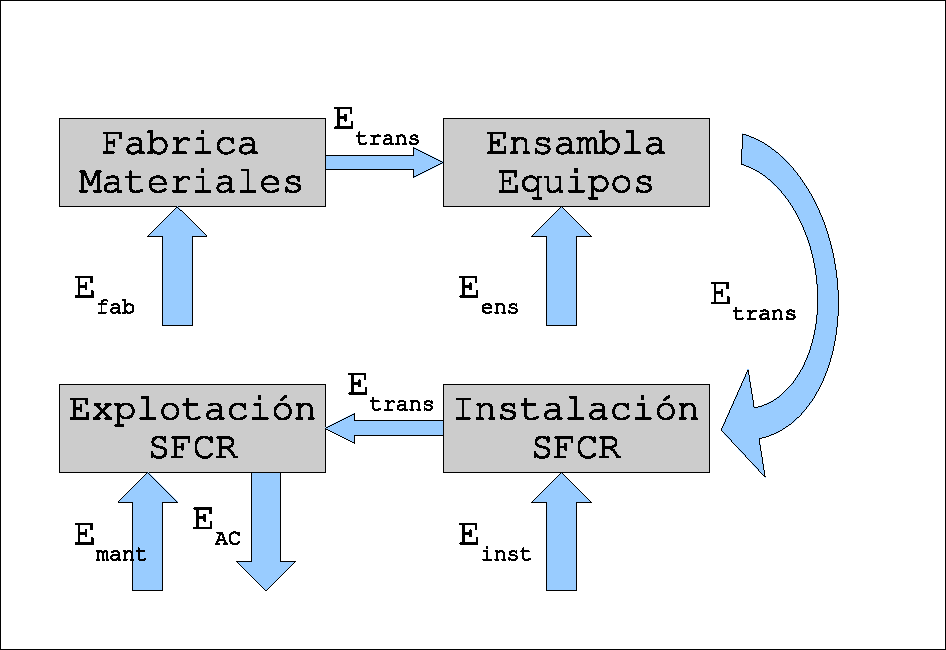
\includegraphics[width=\textwidth]{../Figuras/LCAFlujo.eps}
  
% \end{frame}

% \begin{frame}
%   \frametitle{Energía de los principales componentes}
%   \framesubtitle{Seguimiento a Doble Eje}
%   \begin{tabular}{lll}
%     \toprule
%     Componente              &  ($MJ_{p}/kWp$)  &  (\%)     \\
%     \midrule
%     Módulo & 41\,819 & 69,54\% \\
%     Estructura Soporte      &  9\,329          &  15,51\%  \\
%     Mecanismos de seguimiento    &  248             &  0,41\%   \\
%     Cimientos (acero)     &  3\,371          &  5,61\%   \\
%     Cimientos (hormigón)  &  2\,445          &  4,07\%   \\
%     Transporte              &  1\,339          &  2,23\%   \\
%     Inversor               &  1,091           &  1,81\%   \\
%     Cableado                 &  497             &  0,83\%   \\
%     \midrule
%     Total                  &  60\,140         &  100\%    \\
%     \bottomrule
%   \end{tabular}

% \end{frame}

% \begin{frame}
%   \frametitle{Energía de los principales componentes}
%   \framesubtitle{Seguimiento de Eje Horizontal NS}
%   \begin{tabular}{lll}
%     \toprule
%     Componente              &  ($MJ_{p}/kWp$)  &  (\%)     \\
%     \midrule
%     Módulo & 41\,819 & 78,67\% \\
%     Estructura Soporte      &  6\,108          &  11,49\%  \\
%     Mecanismos de seguimiento    &  58              &  0,11\%   \\
%     Cimientos (acero)     &  1\,536          &  2,89\%   \\
%     Cimientos (hormigón)  &  1\,281          &  2,41\%   \\
%     Transporte              &  900             &  1,69\%   \\
%     Inversor               &  1\,091          &  2,05\%   \\
%     Cableado                 &  364             &  0,68\%   \\
%     \midrule
%     Total                  &  53\,157         &  100\%    \\
%     \bottomrule
%   \end{tabular}
% \end{frame}

% \begin{frame}
%   \frametitle{Energía de los principales componentes}
%   \framesubtitle{Sistemas Estáticos}
%   \begin{tabular}{lll}
%     \toprule
%     Componente              &  ($MJ_{p}/kWp$)  &  (\%)    \\
%     \midrule
%     Módulo & 41\,819 & 81,99\% \\
%     Estructura Soporte      &  4\,459          &  8,74\%  \\
%     Mecanismos de seguimiento    &  0               &  0,00\%  \\
%     Cimientos (acero)     &  0               &  0,00\%  \\
%     Cimientos (hormigón)  &  2\,352          &  4,61\%  \\
%     Transporte              &  1\,037          &  2,03\%  \\
%     Inversor               &  1\,091          &  2,14\%  \\
%     Cableado                 &  248             &  0,49\%  \\
%     \midrule
%     Total                  &  51\,005         &  100\%   \\
%     \bottomrule
%   \end{tabular}
% \end{frame}

% \begin{frame}
%   \frametitle{Valores de EPBT por sistema}
%   \begin{tabular}{ccccccc}
%     \toprule
%     EPBT & 1st. Quartile & Median & Mean & 3rd Quartile \tabularnewline
%     \midrule 
%     Doble Eje & 2,4 & 2,6 & 2,7 & 2,82\tabularnewline
%     Horizontal-NS &  2,65 & 2,88 & 3 & 3,17\tabularnewline
%     Estático & 3 & 3,22 & 3,3 & 3,45\tabularnewline
%     \bottomrule 
%   \end{tabular}

% \end{frame}

% \begin{frame}
%   \frametitle{Doble Eje}
%   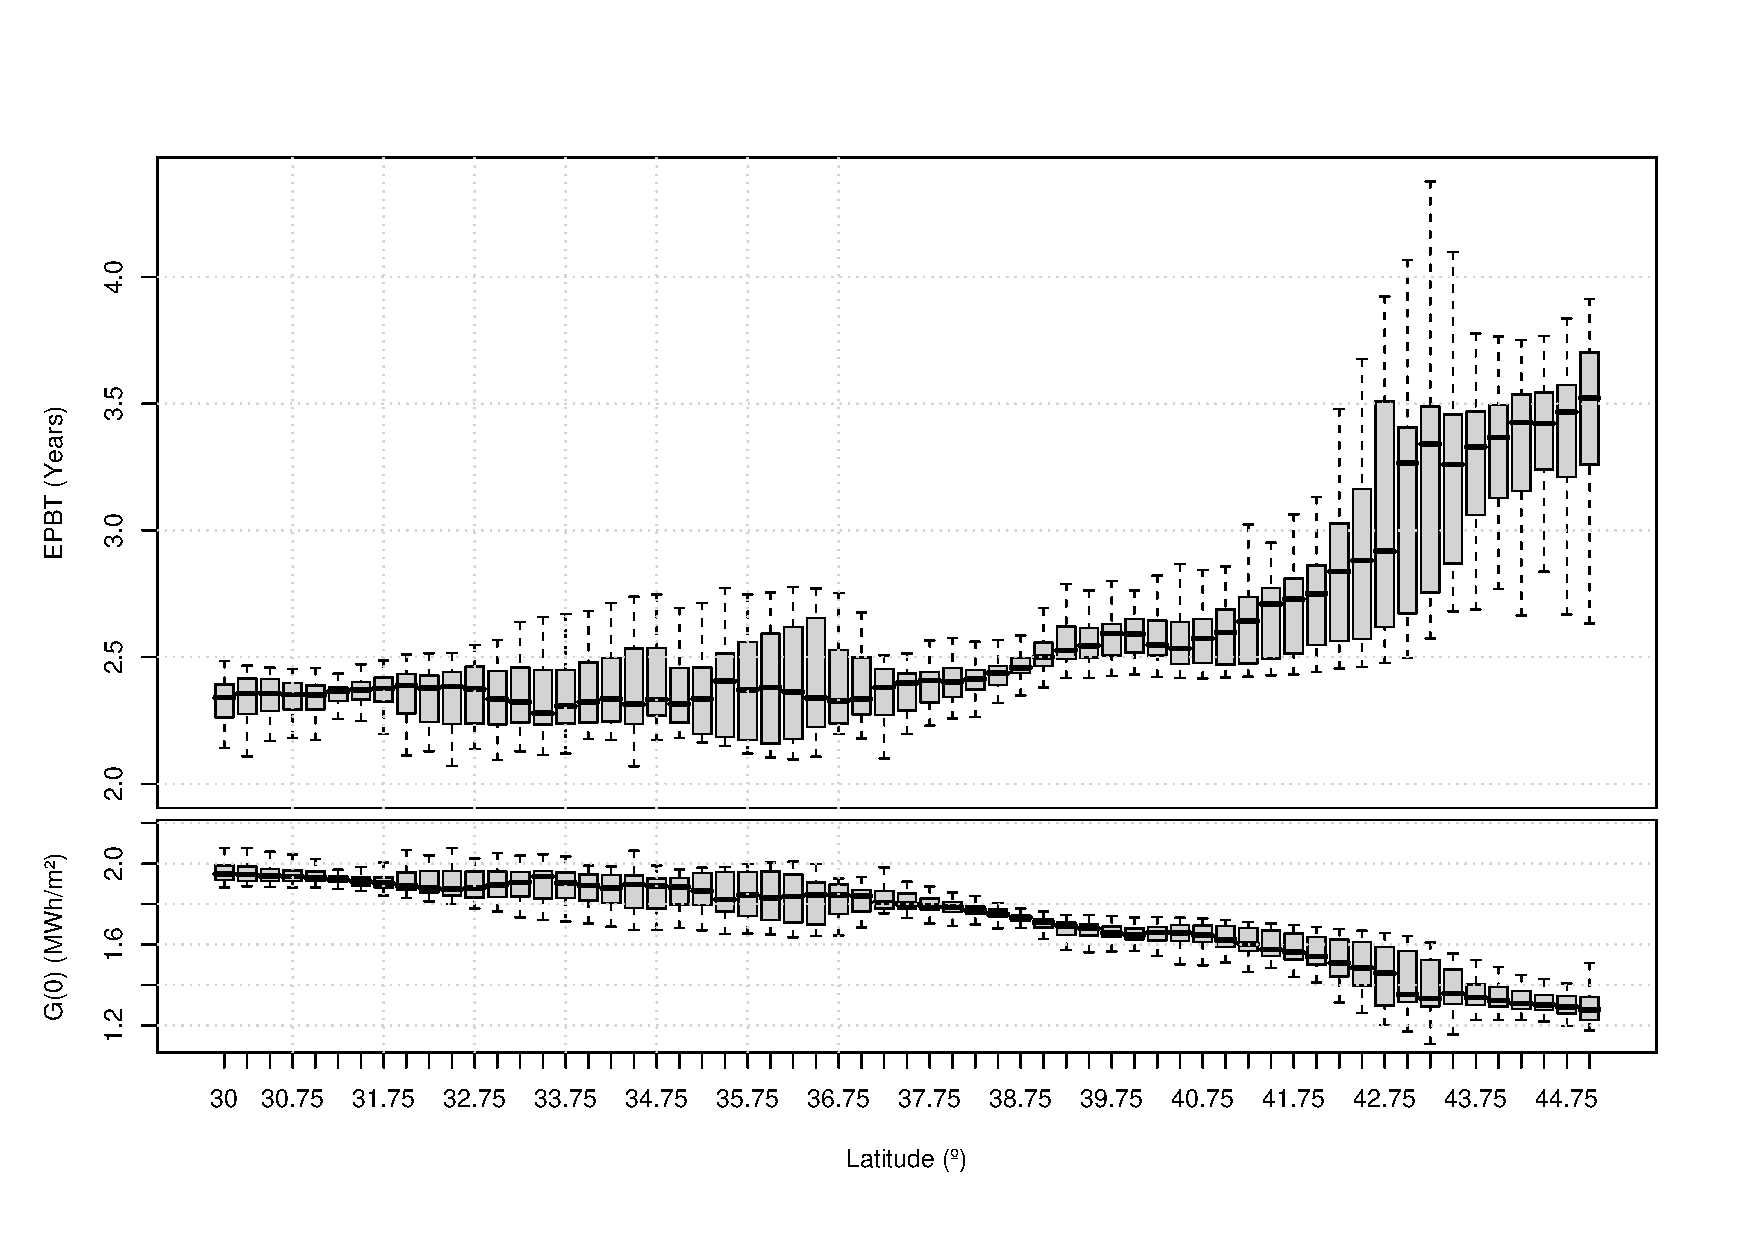
\includegraphics[width=\textwidth]{../Figuras/BoxPlotEPBTEuropa_2x}
% \end{frame}

% \begin{frame}
%   \frametitle{Horizontal NS}
%   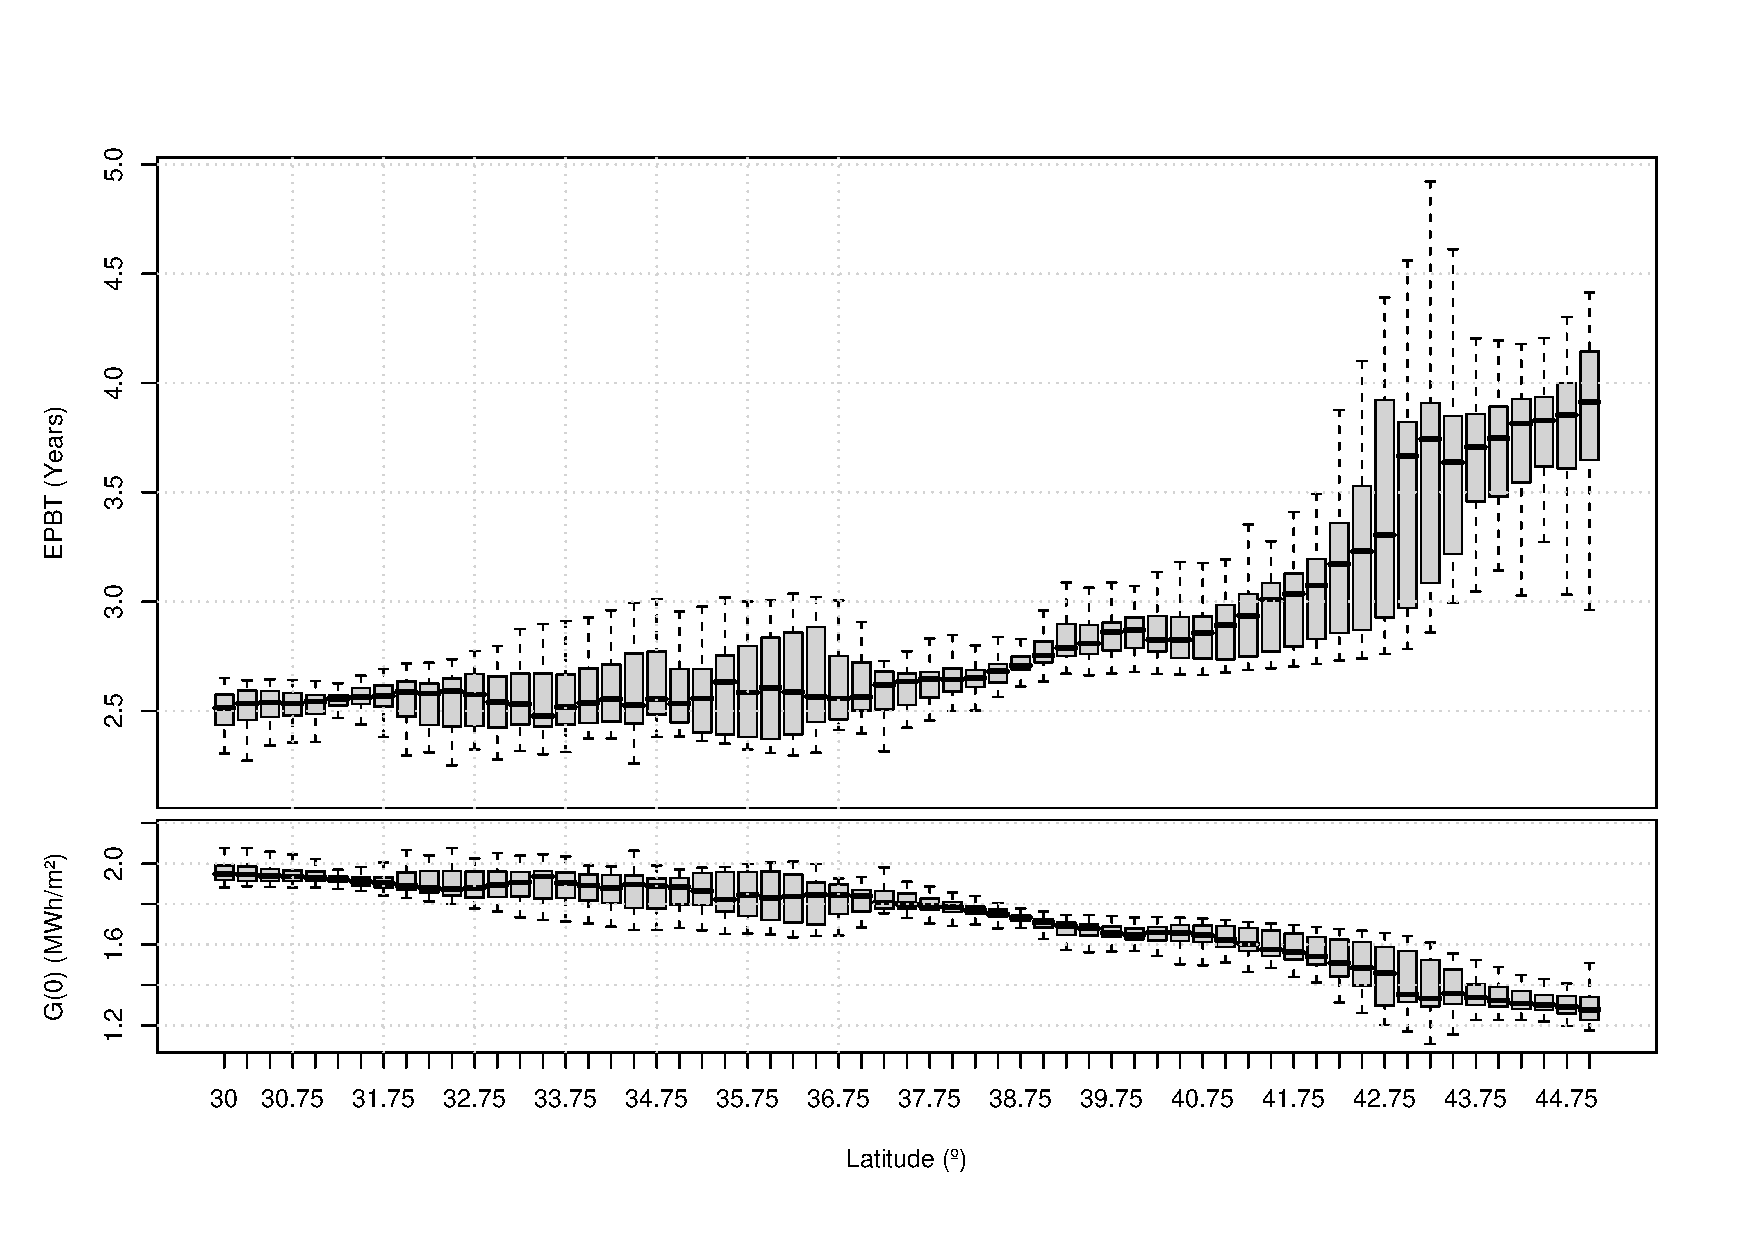
\includegraphics[width=\textwidth]{../Figuras/BoxPlotEPBTEuropa_HorizNS}
% \end{frame}

% \begin{frame}
%   \frametitle{Estático}
%   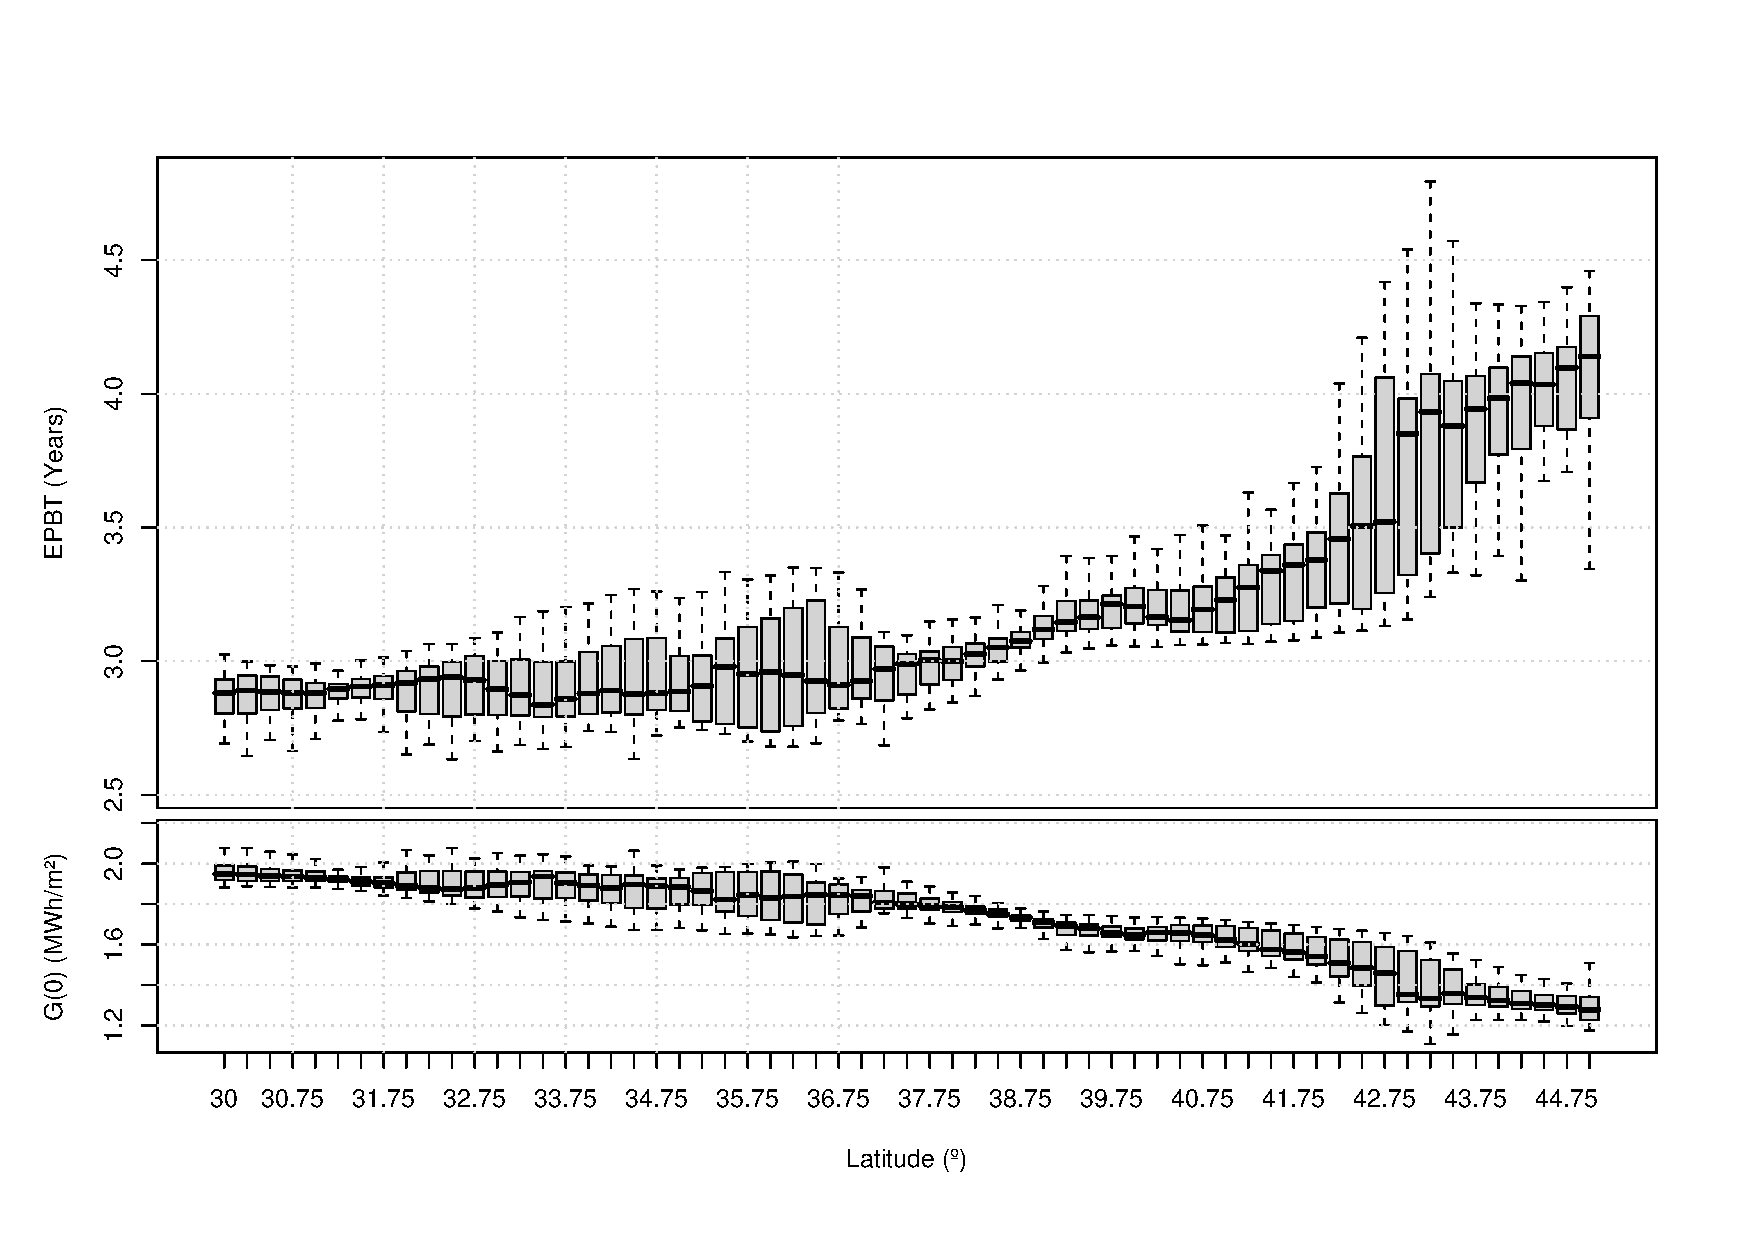
\includegraphics[width=\textwidth]{../Figuras/BoxPlotEPBTEuropa_Fixed}
% \end{frame}

% \begin{frame}
%   \frametitle{Comparativa}
%   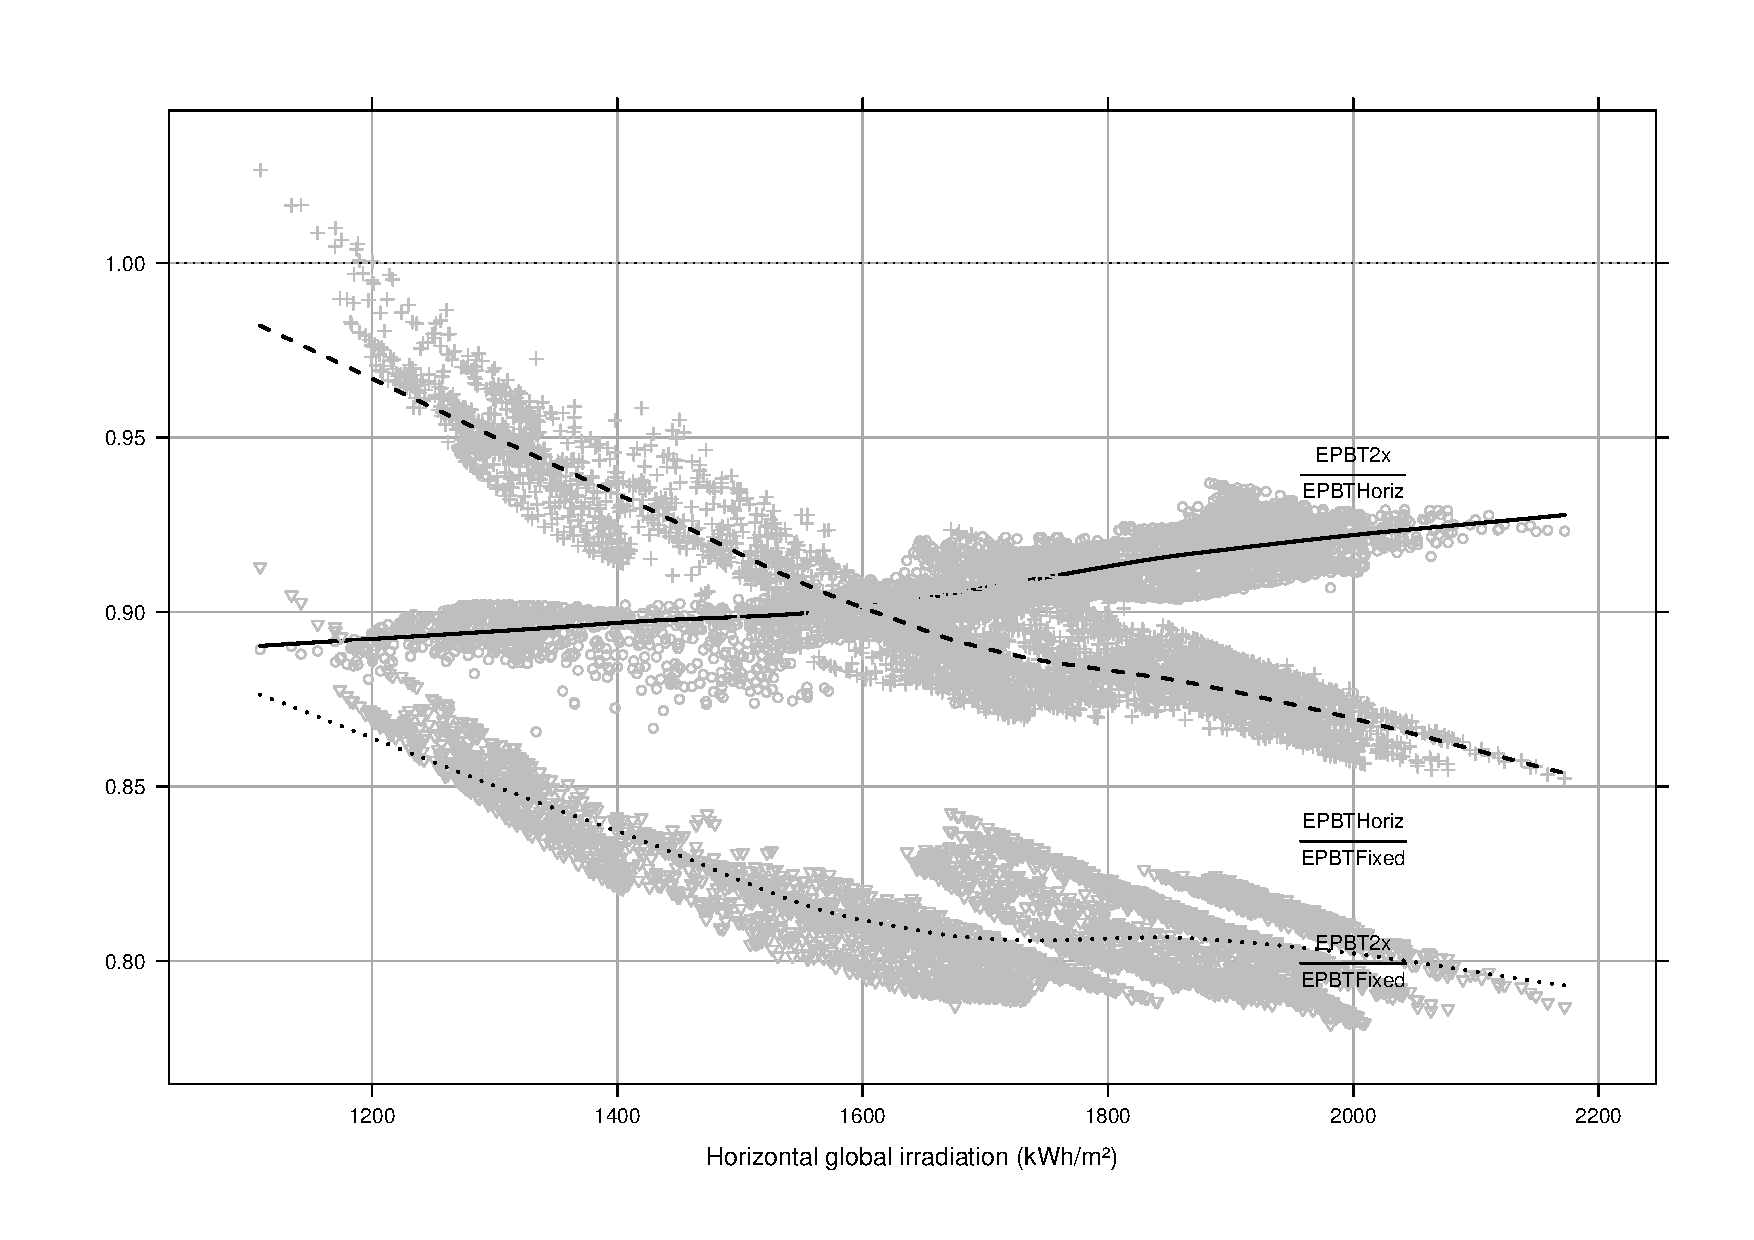
\includegraphics[width=\textwidth]{../Figuras/EPBTEuropavsGh2}
% \end{frame}

\section{Sombras y ocupación de terreno}

\subsection{Sombras Lejanas}


\begin{frame}[plain]
  \frametitle{Método CTE}

  \begin{center}
    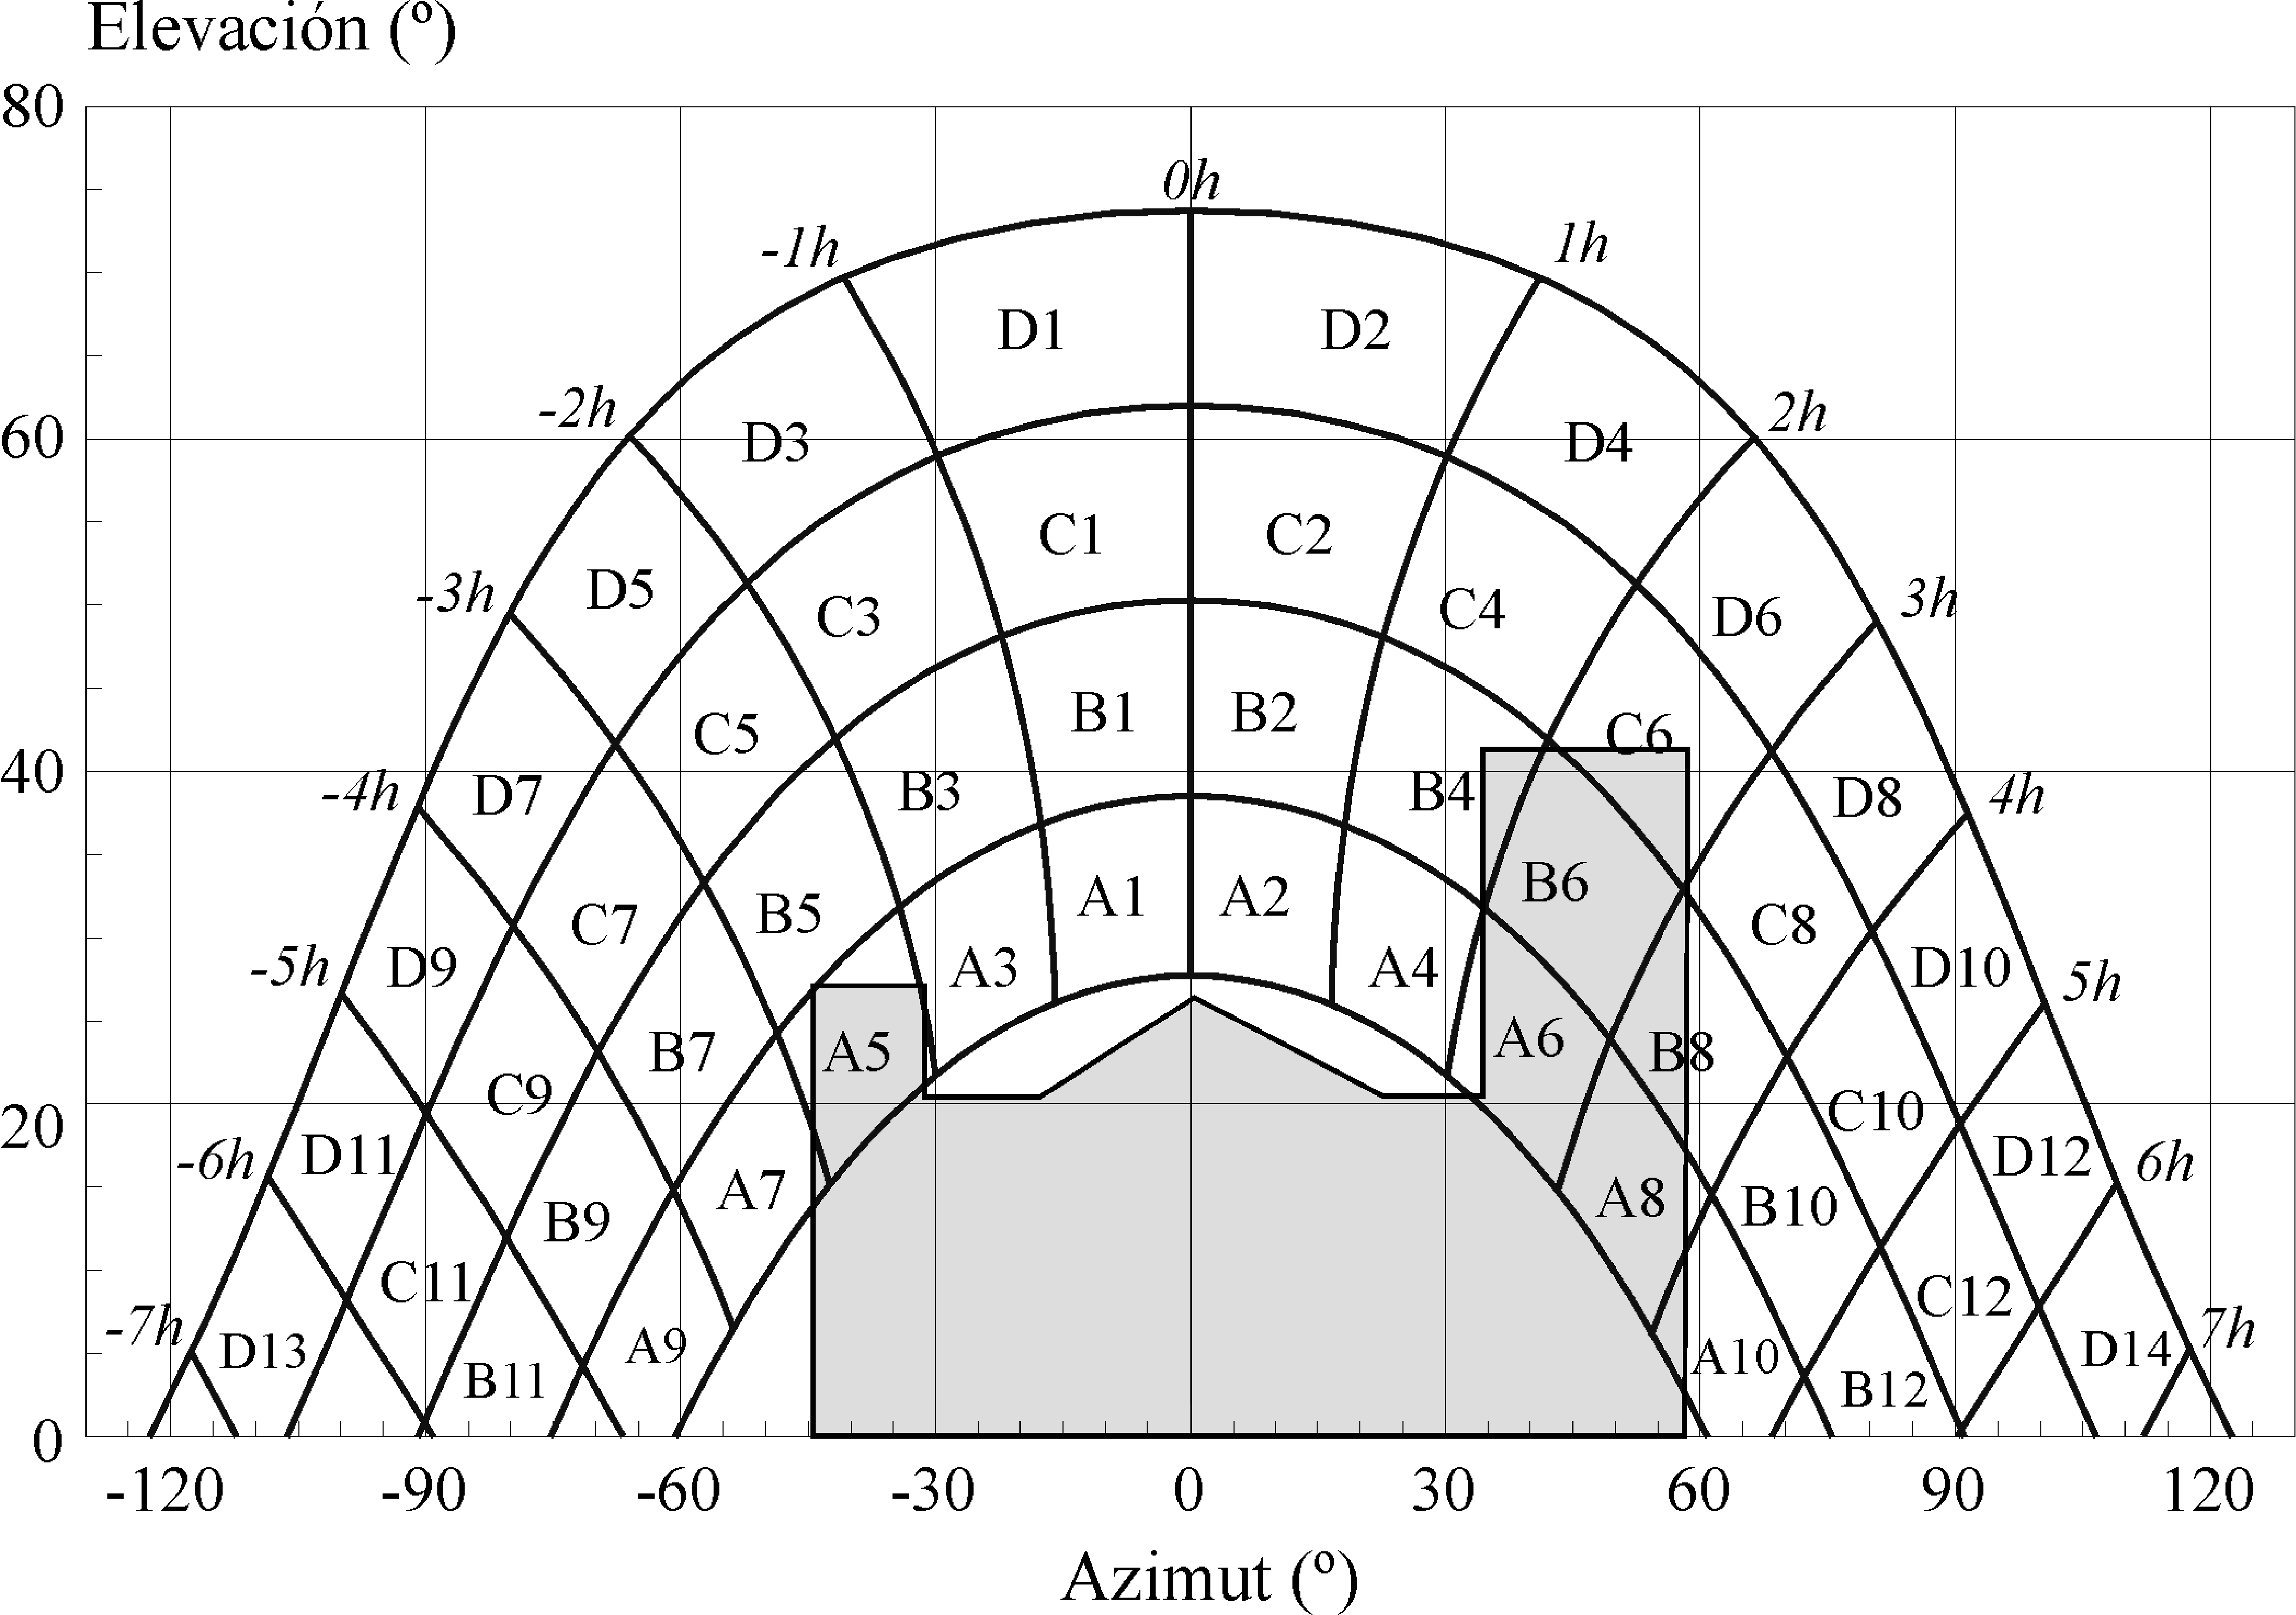
\includegraphics[clip,scale=0.15]{../Figuras/Figuras_Externas/SombraIES}
    \par\end{center}


\end{frame}

\subsection{Sombras Cercanas: sistemas estáticos}


\begin{frame}
  \frametitle{Sombras entre filas}

  \begin{center}
    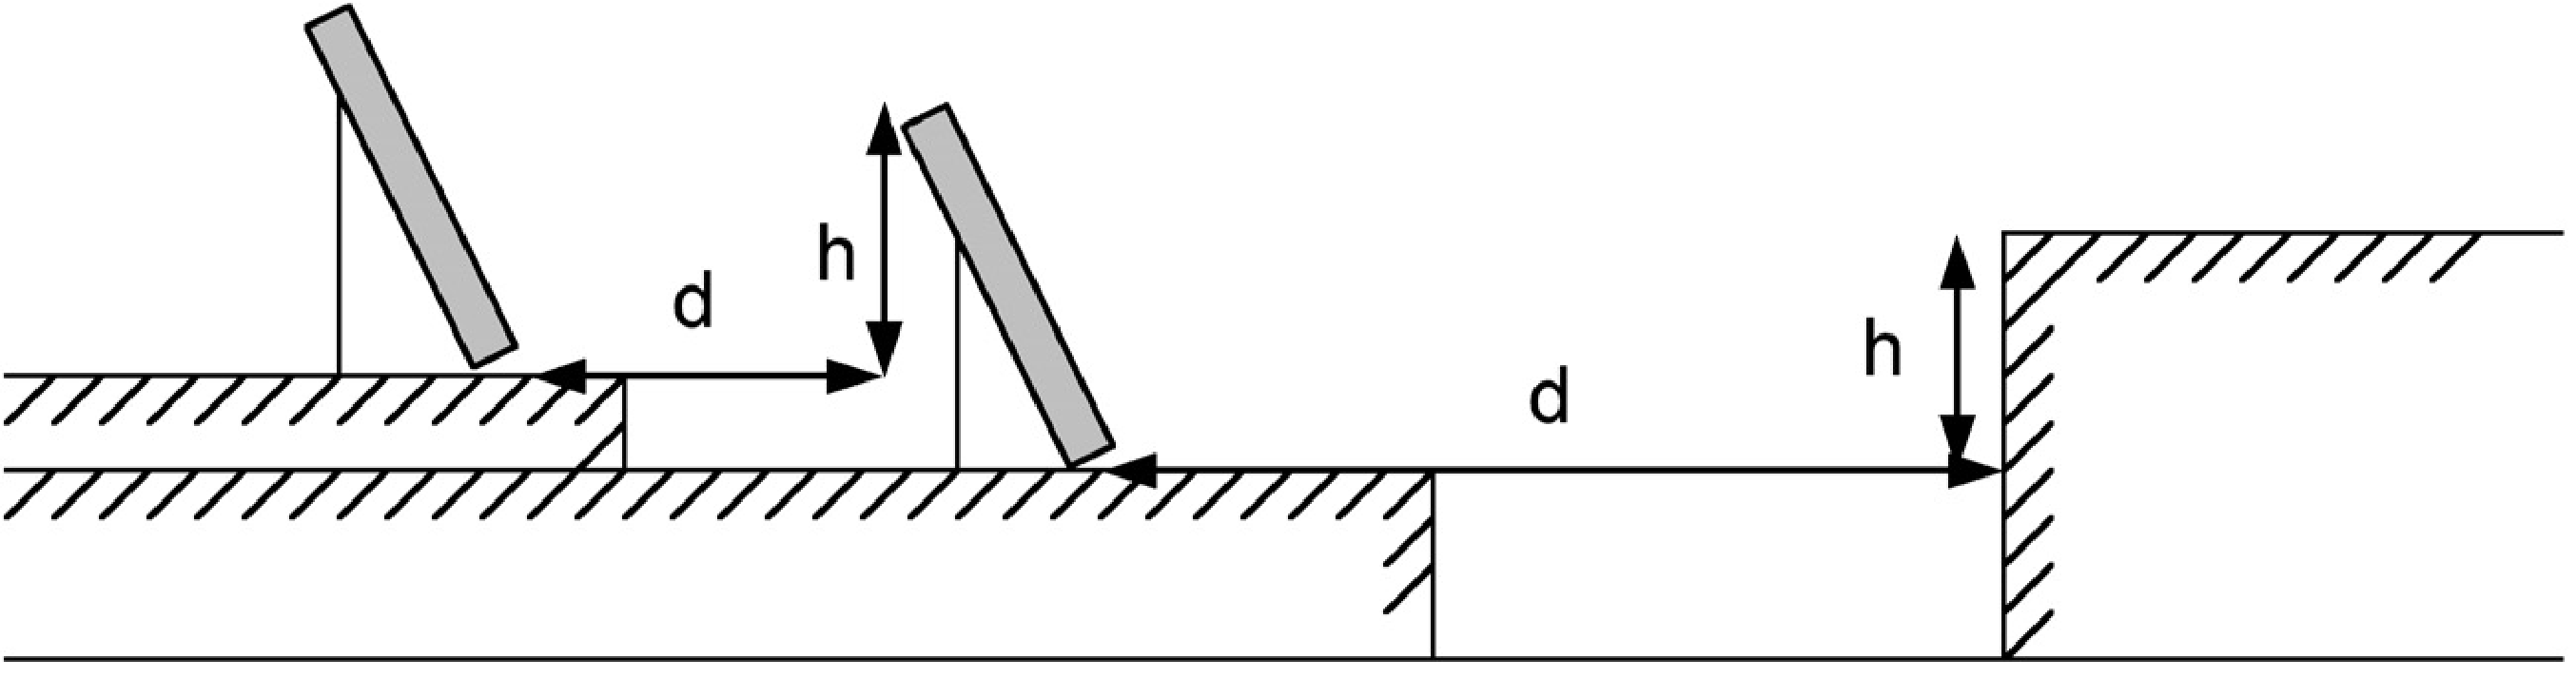
\includegraphics[clip,scale=0.25]{../Figuras/Figuras_Externas/SombraEstaticaInclinado2}
    \par\end{center}
\end{frame}

\begin{frame}
  \frametitle{Sombras entre filas}

  Suele establecerse un objetivo de \textbf{4 horas de sol en torno al
    mediodía del solsticio de invierno libres de sombra}.

  La longitud de la sombra de un obstáculo se mide con:\[
  d=\frac{h}{\tan\gamma_{s}}\]


  En el mediodía del solsticio de invierno \[
  \gamma_{s}=90-23.45-\phi\simeq67-\phi\] Para 2 horas antes y
  después:

\[
d_{min}=\frac{h}{\tan(61\degree-\phi)}\]

\end{frame}

\subsection{Sombras Cercanas: sistemas de seguimiento}


\begin{frame}
  \frametitle{Separación de seguidores Doble Eje}
  \begin{columns}%{}


    \column{7cm}

    \begin{center}
      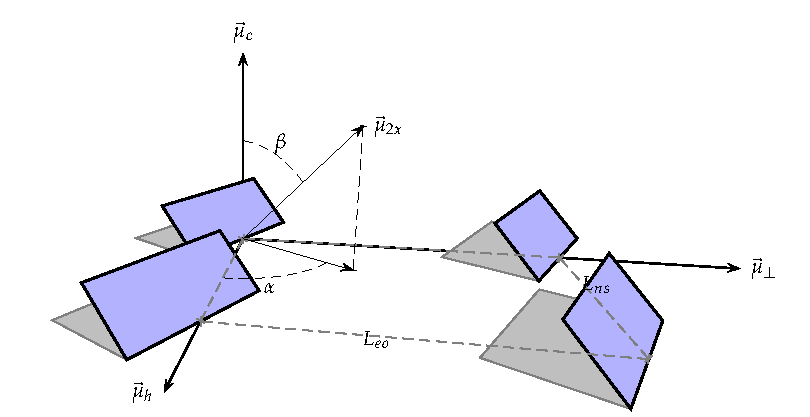
\includegraphics[scale=0.6]{../Figuras/Sombras2X}
      \par\end{center}


    \column{3cm}

    \begin{center}
      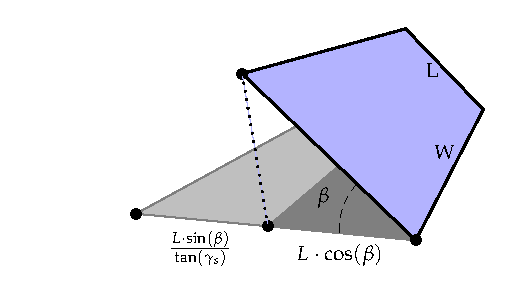
\includegraphics[scale=0.45]{../Figuras/DimensionesSeguidorSombra}
      \par\end{center}

  \end{columns}%{}
  \[
  b=\frac{L}{W}\]
  \[
  ROT=\frac{L_{ns}\cdot L_{eo}}{b}\]


  {\large \[ E_{ac}=f(ROT)??\] }{\large \par}

\end{frame}


\begin{frame}[plain]
\frametitle{Separación de Seguidores Doble Eje}
\begin{columns}[t]%{}


\column{4cm}

{\footnotesize \[
b=\frac{L}{W}=0.475\]
}{\footnotesize \par}


\column{4cm}

{\footnotesize \[
ROT=\frac{L_{ns}\cdot L_{eo}}{b}\]
}{\footnotesize \par}

\end{columns}%{}
\begin{center}
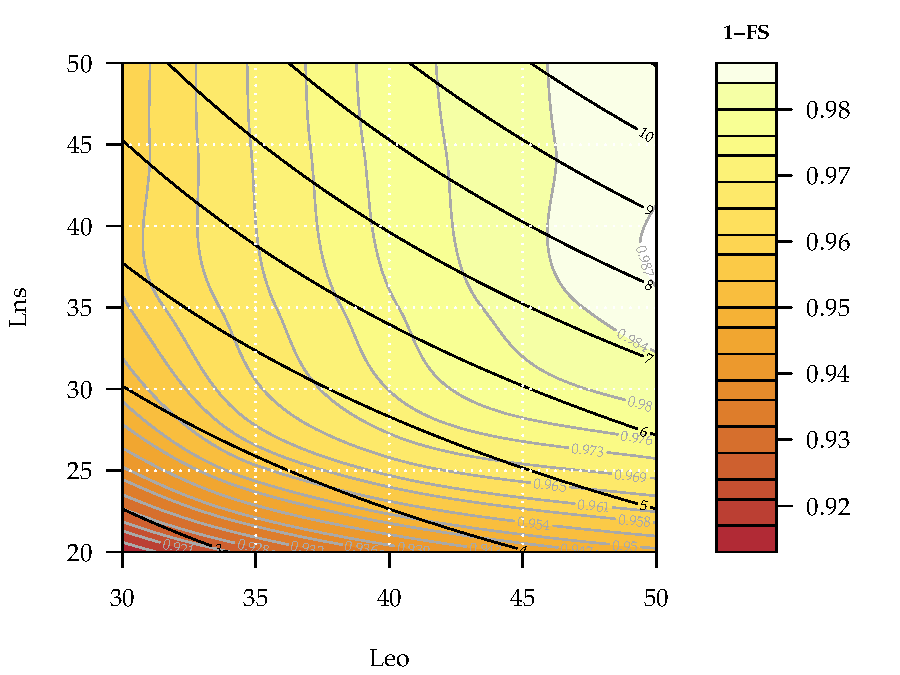
\includegraphics[scale=0.65]{../Figuras/AbacoSeguidor2X_Ene10}
\par\end{center}


\end{frame}

\begin{frame}[plain]
\frametitle{Ocupación de Terreno}


\framesubtitle{ROT para diferentes valores de Leo}
\begin{columns}[t]%{}


\column{4cm}

{\footnotesize \[
b=\frac{L}{W}=0.475\]
}{\footnotesize \par}


\column{4cm}

{\footnotesize \[
ROT=\frac{L_{ns}\cdot L_{eo}}{b}\]
}{\footnotesize \par}

\end{columns}%{}
\begin{center}
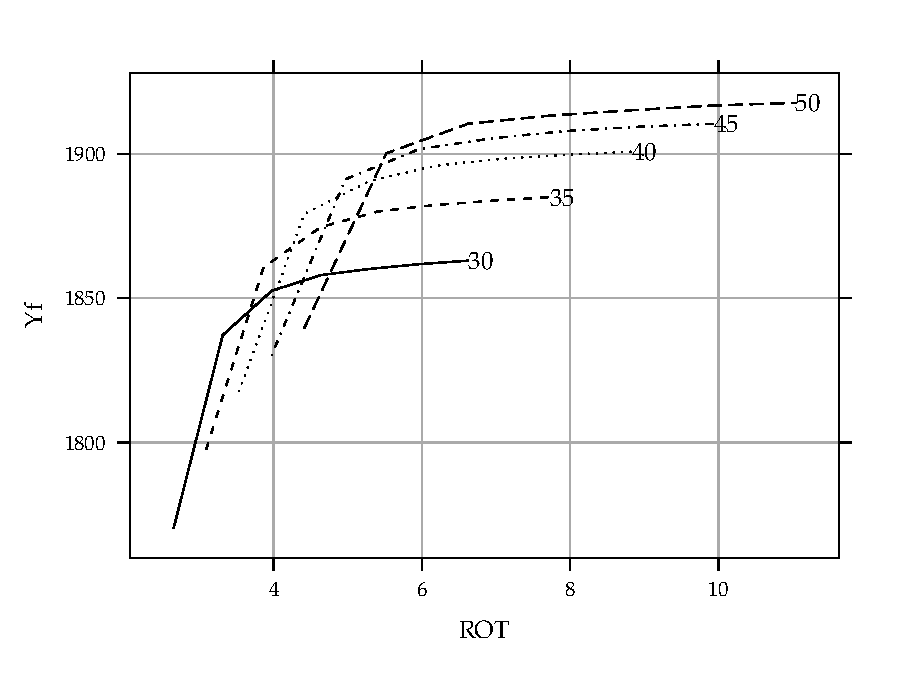
\includegraphics[scale=0.65]{../Figuras/AbacoSeguidor2X_Leo_Ene10}
\par\end{center}


\end{frame}

\begin{frame}[plain]
\frametitle{Ocupación de Terreno}


\framesubtitle{ROT para diferentes valores de Lns}
\begin{columns}[t]%{}


\column{4cm}

{\footnotesize \[
b=\frac{L}{W}=0.475\]
}{\footnotesize \par}


\column{4cm}

{\footnotesize \[
ROT=\frac{L_{ns}\cdot L_{eo}}{b}\]
}{\footnotesize \par}

\end{columns}%{}
\begin{center}
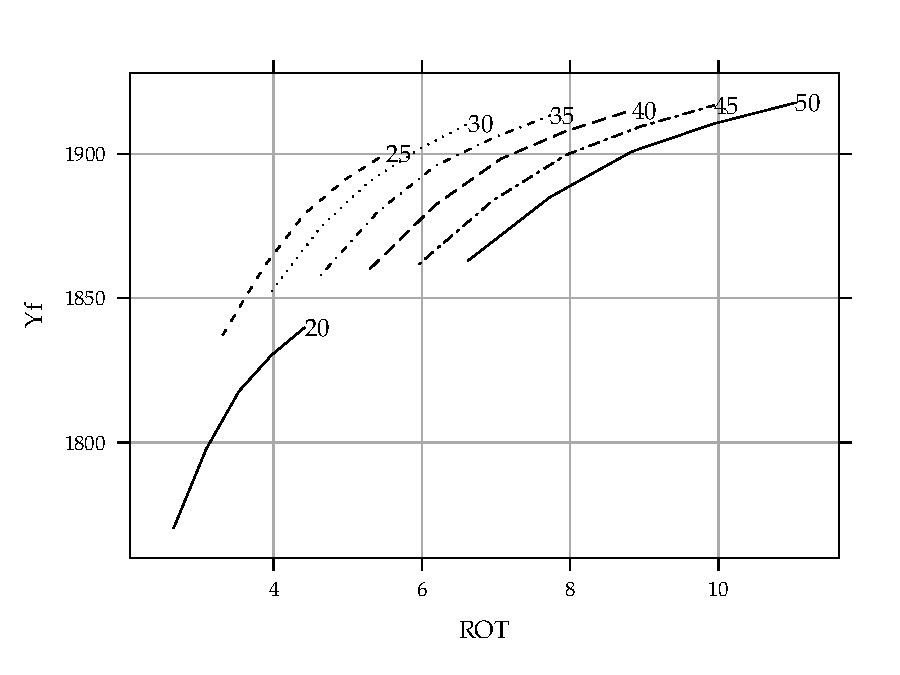
\includegraphics[scale=0.65]{../Figuras/AbacoSeguidor2X_Lns_Ene10}
\par\end{center}


\end{frame}

\subsection{Seguidores de eje horizontal NS}


\begin{frame}
\frametitle{Separación de Seguidores Eje Horizontal}
\begin{columns}%{}


\column{5cm}

\begin{center}
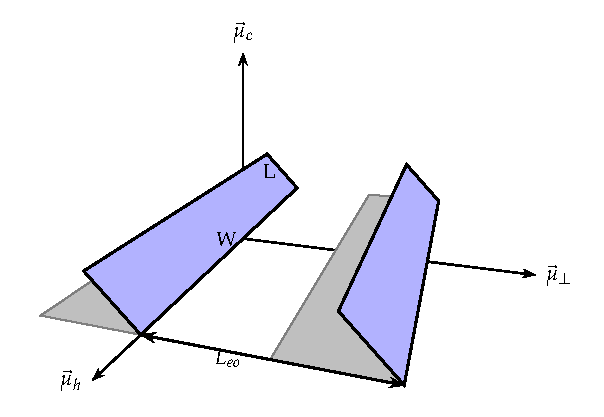
\includegraphics[scale=0.75]{../Figuras/SombrasHoriz}
\par\end{center}


\column{3cm}

\[
W=\infty\]
\[
ROT=L_{eo}/L\]


\end{columns}%{}

\end{frame}

\begin{frame}
\frametitle{Separación de Seguidores Horizontal N-S}


\framesubtitle{Sombra}

\begin{center}
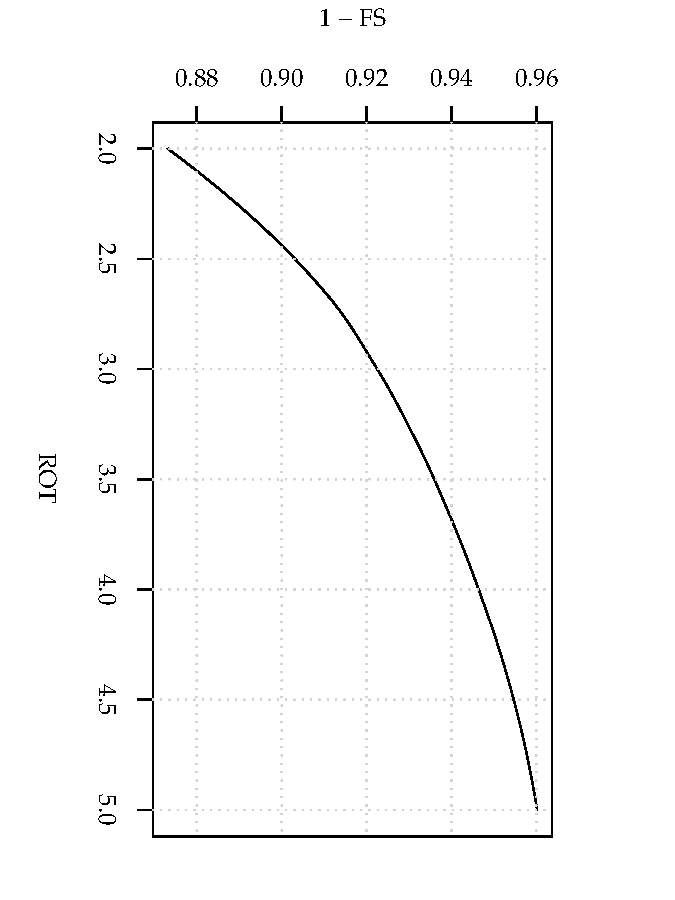
\includegraphics[scale=0.60, angle=90]{../Figuras/AbacoSeguidorHorizSombra_Ene10}
\par\end{center}


\end{frame}

\begin{frame}
\frametitle{Backtracking}
\begin{itemize}
\item El \textbf{sombreado} en un generador puede producir problemas por
el efecto de \textbf{punto caliente}.
\item En seguidores de eje horizontal se puede \textbf{evitar la incidencia
de sombras} en cualquier instante mediante el {}``\textbf{backtracking}'':

\begin{itemize}
\item Al \textbf{amanecer} el seguidor está en posición \textbf{horizontal}.
\item Según avanza el día el seguidor gira en \textbf{sentido contrario
al movimiento solar para evitar las sombras}.
\item En un determinado momento se cruza con el sol y puede continuar el
movimiento {}``convencional''.
\item En un instante de la tarde debe volver a cambiar el sentido hasta
la \textbf{horizontal en la noche}.
\end{itemize}
\end{itemize}

\end{frame}

\begin{frame}
\frametitle{Backtracking}

\begin{center}
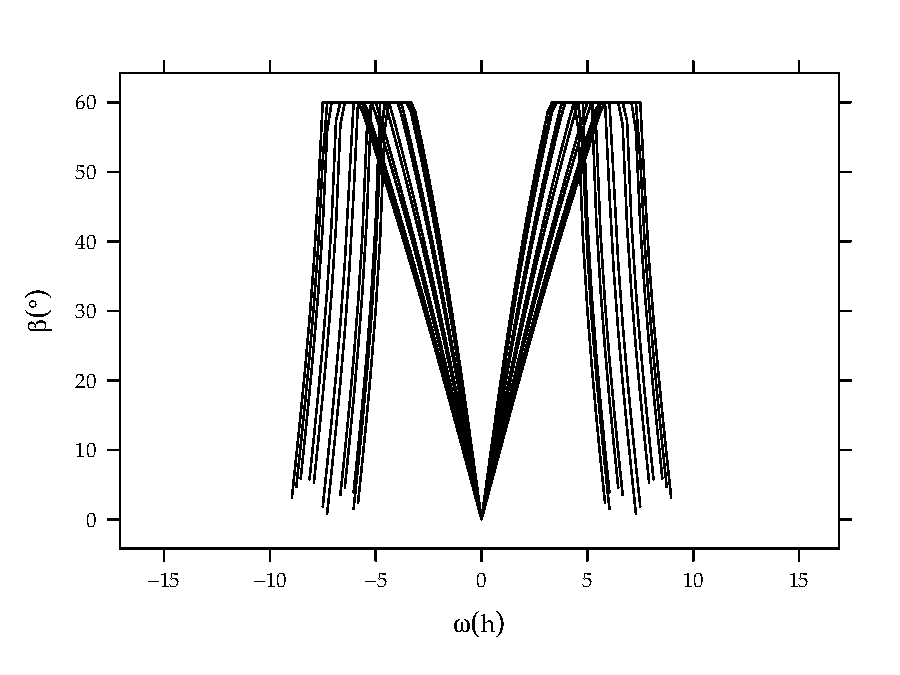
\includegraphics[scale=0.62]{../Figuras/BackTracking}
\par\end{center}


\end{frame}

\begin{frame}
\frametitle{Separación de Seguidores Horizontal N-S}


\framesubtitle{Backtracking}

\begin{center}
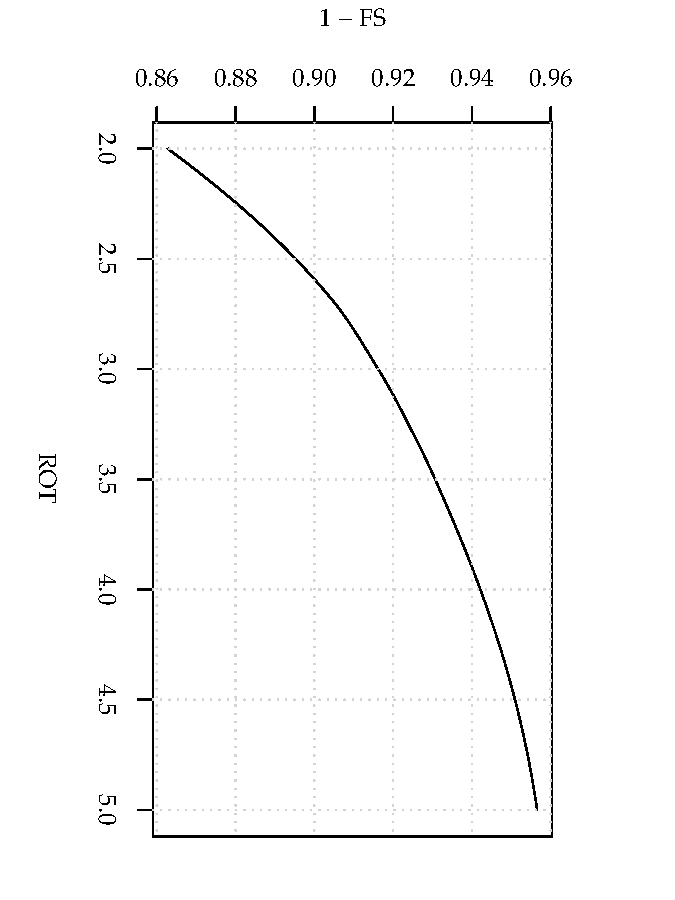
\includegraphics[scale=0.60, angle=90]{../Figuras/AbacoHorizBT_Ene10}
\par\end{center}


\end{frame}

\subsection{Elección de separaciones}


\begin{frame}
\frametitle{Elección de separaciones}
\begin{block}
{Elección de separaciones}

La \textbf{separación óptima} entre elementos (seguidores o estructuras
estáticas) es aquella que conduce al \textbf{mínimo valor del coste
de la energía} producida por el sistema:
\begin{itemize}
\item Con mayor separación disminuyen las \textbf{pérdidas por sombreado
mutuo}, aumenta la productividad del sistema.
\item Con mayor separación aumentan los \textbf{costes relacionados con
el area ocupada} por unidad de potencia.
\item Con mayor separación aumentan los \textbf{costes relacionados con
los elementos de unión entre estructuras} (cableado, canalizaciones,
zanjas).
\end{itemize}
\end{block}

\end{frame}

\begin{frame}
\frametitle{Elección de separaciones}
\begin{block}
{}
\begin{itemize}
\item Esta separación óptima \textbf{depende} de las \textbf{estructuras
elegidas} y de las \textbf{condiciones económicas} de los elementos. 
\item La separación finalmente elegida debe \textbf{tomar en consideración
las condiciones del terreno} (fronteras, irregularidades, vaguadas,
etc.)
\end{itemize}
\end{block}

\end{frame}

\begin{frame}[plain]
  \frametitle{Radiación promedio}

  \begin{equation*}
    G_{ef, av} = 1/24 \cdot \left( 10 \cdot G_{ef,0} + 5 \cdot G_{ef,A}
      + G_{ef,B} + 2 \cdot G_{ef,C} + G_{ef,D} + 5 \cdot G_{ef,E} \right)
  \end{equation*}

  \begin{columns}

    \begin{column}{4cm}
      \begin{center}
        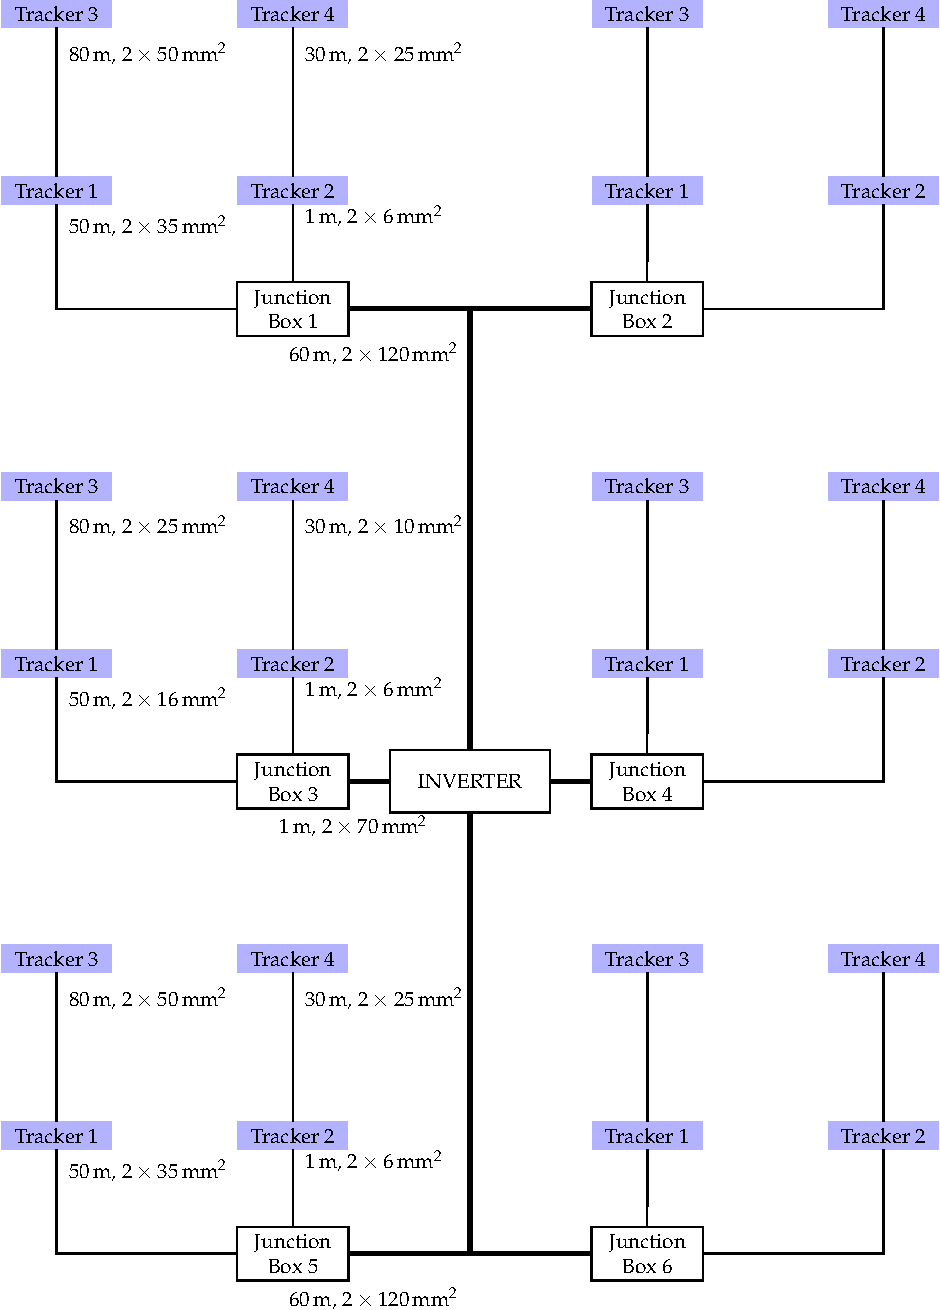
\includegraphics[scale=0.28]{../Figuras/plantConfiguration}
      \end{center}
    \end{column}

    \begin{column}{6cm}
      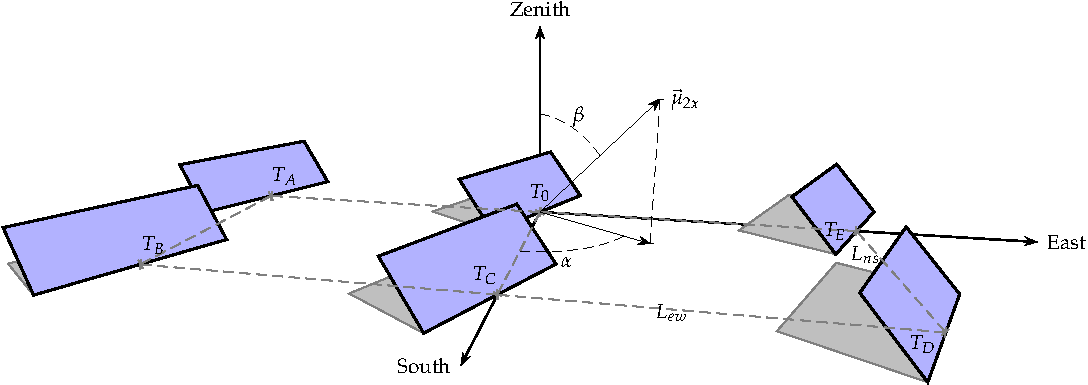
\includegraphics[scale=0.4]{../Figuras/6trackers}

    \end{column}
  \end{columns}


\end{frame}

\begin{frame}[plain]
  \frametitle{Cableado}

  \begin{center}
    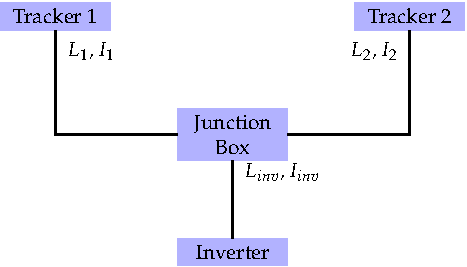
\includegraphics[scale=0.6]{../Figuras/wiring}
  \end{center}

  \begin{align*}
    \Delta U_{inv} &= \frac{\Delta U}{1+\sqrt{\frac{\sum_{i=1}^n
          L_{i}^2 \cdot I_{i}}{L_{inv}^2 \cdot I_{inv}}}} \\
    \Delta U_{inv} &+ \Delta U_i = \Delta U\\
    S_{inv} &= 2 \cdot \rho \cdot \frac{L_{inv} \cdot
      I_{inv}}{\Delta U_{inv}} \\
    S_{i} &= 2 \cdot \rho \cdot \frac{L_{i} \cdot I_i}{\Delta U_i}
  \end{align*}


\end{frame}

\begin{frame}[plain]
  \frametitle{Coste de la energía producida}

  \begin{align*}
    C_E &= \frac{C_P}{E_{AC}}\\
    C_p &= C_c + C_A + C_{PV}
  \end{align*}

  \begin{columns}
    \begin{column}{5cm}
      \begin{center}
        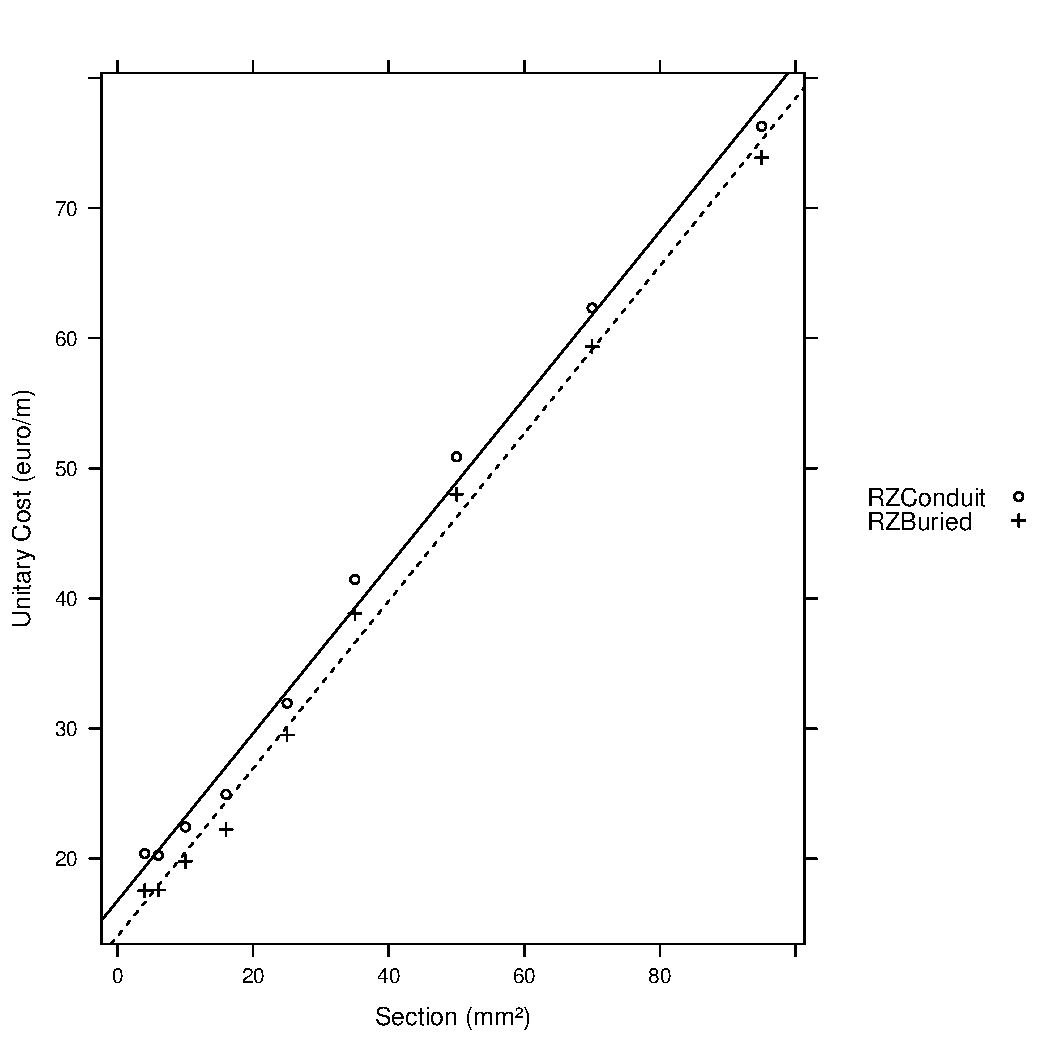
\includegraphics[scale=0.3]{../Figuras/WiringCosts.pdf}
      \end{center}
    \end{column}
    \begin{column}{5cm}
      $C_{PV}$ entre $\SI{2.5}{\text{\texteuro}\per\watt}$ y
      $\SI{5}{\text{\texteuro}\per\watt}$

      $C_A$ entre $\SI{1.5}{\text{\texteuro}\per\meter\squared}$ y
      $\SI{4}{\text{\texteuro}\per\meter\squared}$
    \end{column}

  \end{columns}



\end{frame}

\begin{frame}[plain]
%  \frametitle{Resultados}
  \begin{center}
      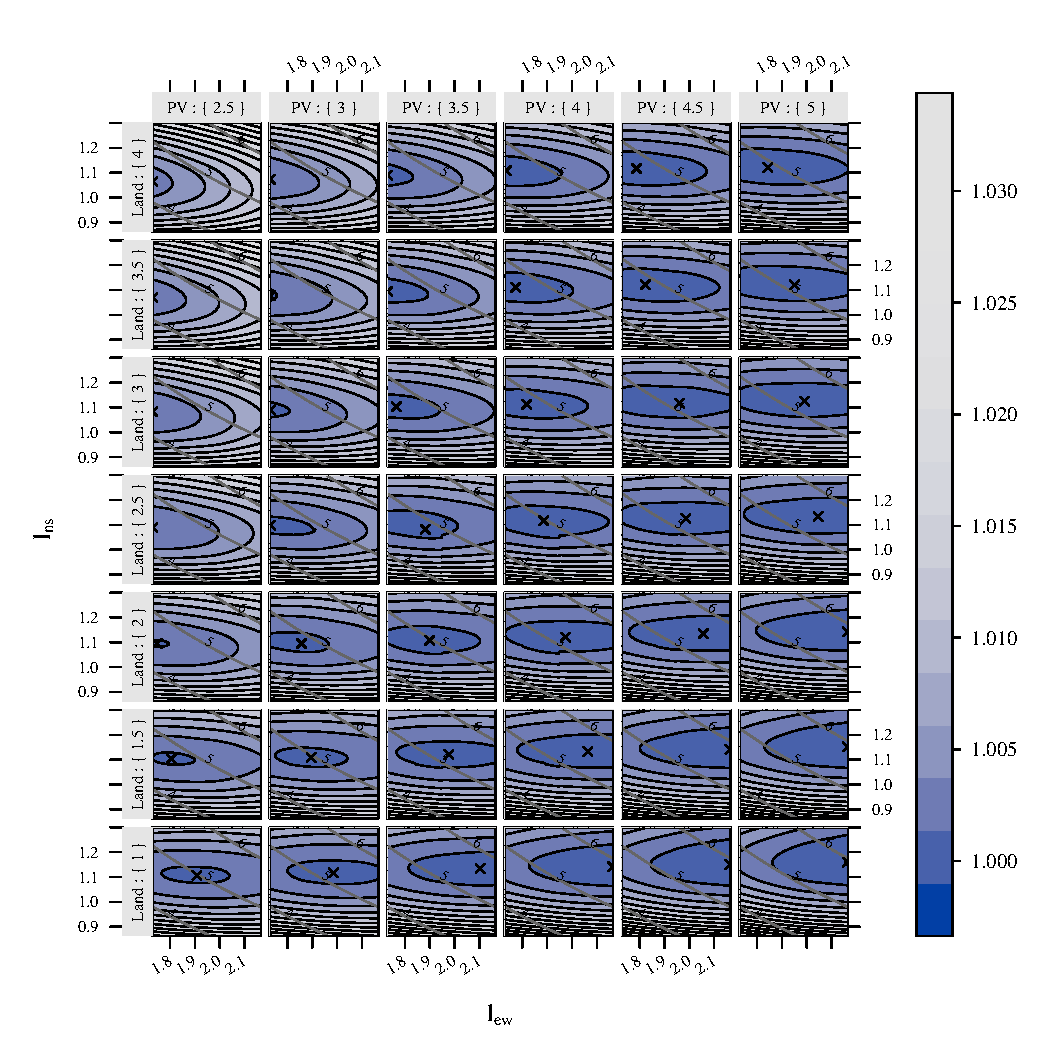
\includegraphics[scale=0.53]{../Figuras/matrix-300dpi}
  \end{center}
\end{frame}

\begin{frame}[plain]
  \frametitle{Resultados}
  \begin{center}
      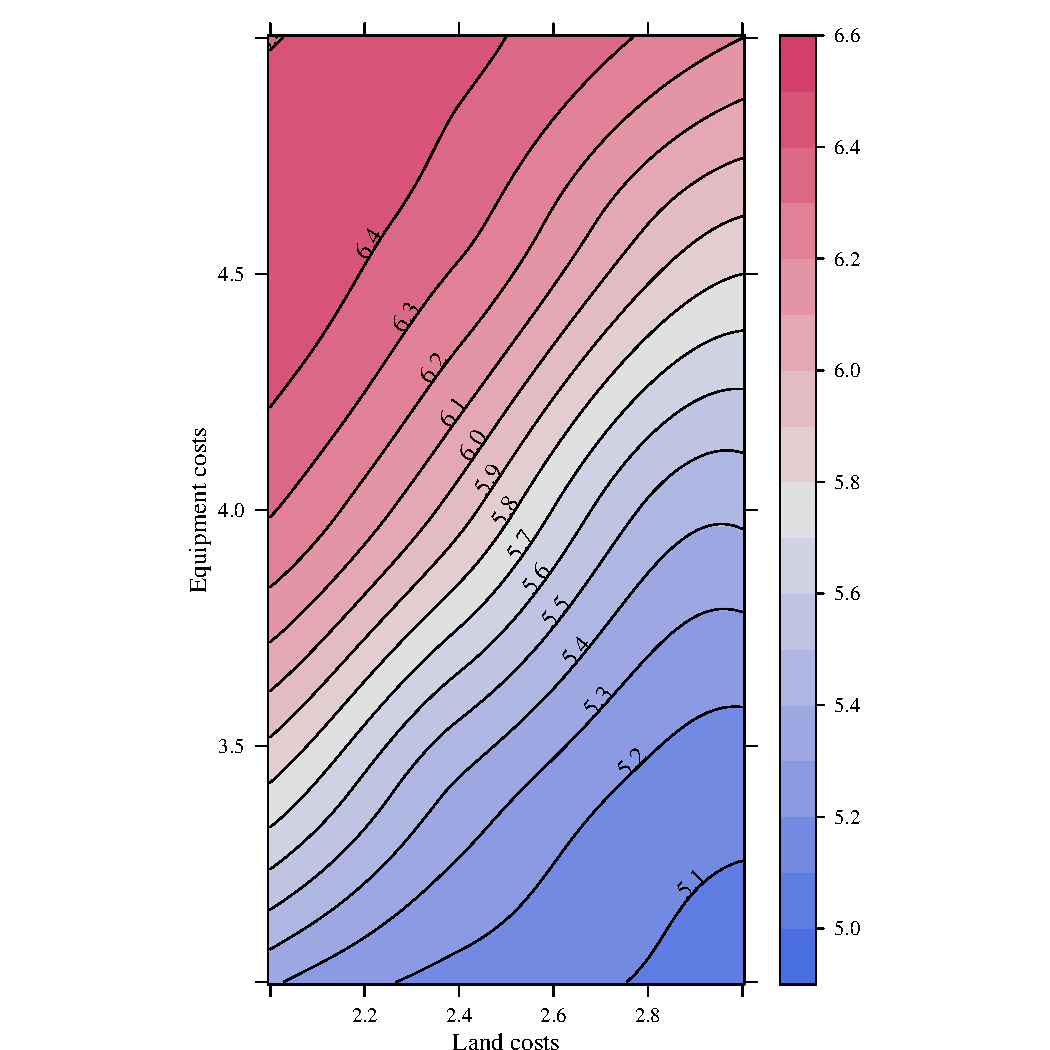
\includegraphics[scale=0.45]{../Figuras/GRRoptim}
  \end{center}
\end{frame}


\section{Resumen}

\begin{frame}
\frametitle{Ocupación de terreno y productividad}
\begin{block}
{}

\begin{center}
\begin{tabular}{ccc}
\toprule 
SFCR & ROT & Productividad\tabularnewline
\midrule
\midrule 
Estático & 2 & 1\tabularnewline
\midrule 
Eje Horizontal NS & 4 & 1,05-1,2\tabularnewline
\midrule 
Doble Eje & 6 & 1,3-1,5\tabularnewline
\bottomrule
\end{tabular}
\par\end{center}

\end{block}

\end{frame}

\end{document}
